\title{ICP473 - Segurança da Informação}

\author{Prof. Gabriel Rodrigues Caldas de Aquino}

\institute
{
    Instituto de Computação \\
    Universidade Federal do Rio de Janeiro\\
    gabrielaquino@ic.ufrj.br% Your institution for the title page
}
\date{Compilado em: \\ \today} % Date, can be changed to a custom date

%----------------------------------------------------------------------------------------
%    PRESENTATION SLIDES
%----------------------------------------------------------------------------------------



\begin{frame}
    % Print the title page as the first slide
    \titlepage
\end{frame}




\begin{frame}{Livros Base}
\centering
\begin{columns}
    \begin{column}{0.5\linewidth}
        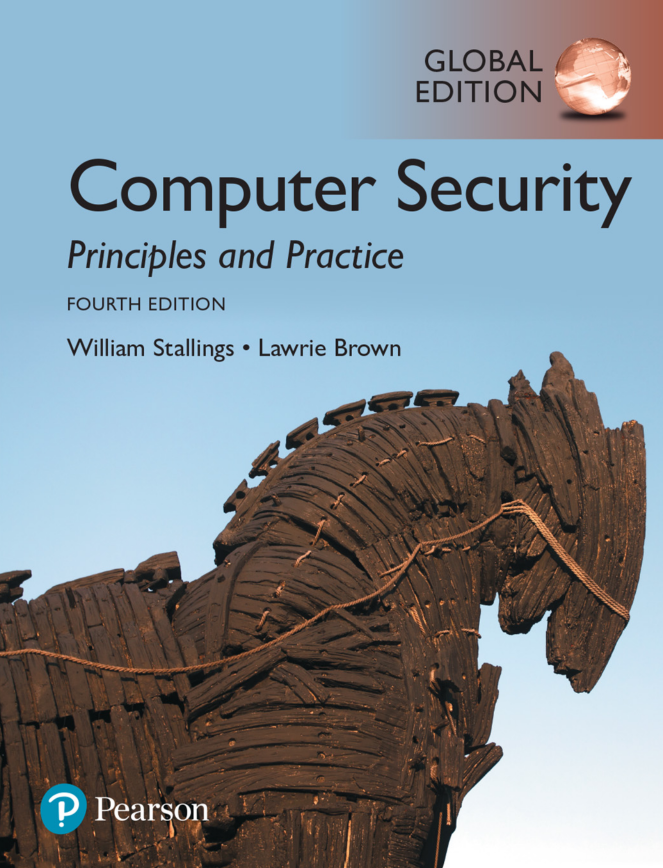
\includegraphics[width=0.8\linewidth]{Figuras/livro-stallings-sec.png}
    \end{column}
    \begin{column}{0.5\linewidth}
        \begin{itemize}
            \item Computer Security - Principles and Practice\\
Fourth Edition \\
Global Edition \\
William Stallings \\ 
Lawrie Brown \\
ISBN 10: 1-292-22061-9\\
ISBN 13: 978-1-292-22061-1
        \end{itemize}
    \end{column}
\end{columns}

\end{frame}

\begin{frame}{Livros Base}
\centering
\begin{columns}
    \begin{column}{0.5\linewidth}
      \begin{itemize}
          \item Criptografia e segurança de redes: princípios e práticas \\ William
Stallings;\\ tradução Daniel Vieira; revisão técnica Paulo Sérgio Licciardi
Messeder Barreto, Rafael Misoczki. – 6. ed. – São Paulo: Pearson
\\Education do Brasil, 2015.
\\Título original: Cryptography and network security
\\ISBN 978-85-430-1450-0
      \end{itemize}
    \end{column}
    \begin{column}{0.5\linewidth}
        
\includegraphics[width=0.8\linewidth]{Figuras/livro-stallings-cripto.png}
    \end{column}
\end{columns}

\end{frame}

\begin{frame}{Método de Avaliação}
  \begin{block}{Componentes da Nota}
    \begin{itemize}
      \item \textbf{Provas (P1 e P2):}  
  Média das provas (MP) $\rightarrow$ 80\% da nota
      \item \textbf{Trabalhos:} 
  Média dos trabalhos (MT) $\rightarrow$ 20\% da nota 
    \end{itemize}
  \end{block}

  \begin{block}{Critério de Aprovação Direta}
    \begin{itemize}
      \item Média ponderada de MP e MT $\geq 7$ 
      \hspace{1em} $\rightarrow$ Aprovado direto
      \item Se $3 <= \text{Média ponderada de MP e MT } <= 7$ 
      \hspace{1em} $\rightarrow$ Prova final (PF)
    \end{itemize}
  \end{block}

  \begin{block}{Cálculo da Média Final}
    \[
      \text{Média final} = \frac{\text{Média anterior} + \text{PF}}{2}
    \]
    \begin{itemize}
      \item Se $\text{Média final} \geq 5$ $\Rightarrow$ Aprovado
      \item Caso contrário $\Rightarrow$ Reprovado
    \end{itemize}
  \end{block}
\end{frame}

